\documentclass[Protokollheft.tex]{subfiles}
\begin{document}
\chapter{Einführung in Numerische Methoden}
%--------------- Start Vorbereitungsaufgaben ---------------

\section{Vorbereitungsaufgaben}
    {\subsection{Differenzenverfahren}}

% --> Aufgabe
    \begin{framed}
	\noindent \textbf{1.} Zeigen Sie, dass der zentrale Differenzenquotient (1.5) aus der Subtraktion zweier Taylor-Entwicklungen zu den Punkten $x_{i+1}$ und $x_{i-1}$ folgt. Vergessen Sie dabei nicht, die Fehlerterme zu berücksichtigen und kommentieren Sie die Ordnung des Fehlers im Vergleich zu vorwärts- und rückwärts-Differenzenquotient.\label{exer:diffquot}
\end{framed}

\emph{Fügen Sie hier Ihre Lösung ein}

% --> Aufgabe
    \begin{framed}
	\noindent \textbf{2.} Berechnen Sie ausgehend von einem Startpunkt \(f(\tilde{x}_i)\) auf einem dualen Gitter mit Hilfe von Taylorentwicklungen analog zur Differenzenvorschrift (1.6) im Fall äquidistanter Gitter eine zentrale Differenzenvorschrift vierter Ordnung zur Berechnung der ersten Ableitung. Verwenden Sie hierfür \(f(x_i), f(x_{i+1}), f(x_{i+2})\) sowie \(f(x_{i-1})\).\label{exer:diffquotOrd4}
\end{framed}

\emph{Fügen Sie hier Ihre Lösung ein}

% --> Aufgabe
    \begin{framed}
	\noindent \textbf{3.} Bestimmen Sie aus der Differenzenvorschrift (1.10) die Matrix $\tilde{\textbf{C}}\textbf{C}$ für einen 1D-Resonator mit $5$~Stützstellen für den Fall elektrischer bzw. magnetischer Randbedingungen an beiden Rändern (siehe Abb.~1.3,~Gl.~(1.15)~und~Gl.~(1.16)).\label{exer:matrixCC}
\end{framed}

\emph{Fügen Sie hier Ihre Lösung ein}

% --> Aufgabe
    \begin{framed}
	\noindent \textbf{4.} Betrachtet werden soll exemplarisch die Berechnung der diskreten Wellenzahlen bei vorgegebener Länge des Rechengebietes nach Gl.~(1.14).
    Geben Sie den Abbruchfehler in Abhängigkeit von der Anzahl der verwendeten Stützstellen $n$ bzw. der Diskretisierungsschrittweite $\Delta x$ an,
    wenn der Differenzenquotient nach Gl.~(1.9) bzw. Gl.~(1.10) verwendet wird.
    Wie müssen Sie ein entsprechendes Diagramm (Abbruchfehler vs. Anzahl der Stützstellen) skalieren, um einen geradlinigen Verlauf zu erhalten?\label{exer:failureTerm}
\end{framed}

\emph{Fügen Sie hier Ihre Lösung ein}

% --> Aufgabe
    \begin{framed}
	\noindent \textbf{5.} Stellen Sie eine Formel auf, mit der die analytischen Wellenzahlen $k_{x,\,\text{ana}}$ für die eindimensionale Wellengleichung und
    einem Resonator der Länge~\(L\) einmal mit rein elektrischer Berandung und einmal mit unterschiedlichen Randbedingungen
    (eine Seite elektrisch -- eine Seite magnetisch) berechnet werden kann. Bestimmen Sie dabei auch die jeweils kleinste Wellenzahl.
    Geben Sie bei einer numerischen Berechnung eine Formel für den relativen Wellenzahlfehler $\Delta k_{x}$ an.\label{exer:kxAnalytic}
\end{framed}

\emph{Fügen Sie hier Ihre Lösung ein}

% --> Aufgabe
    \begin{framed}
	\noindent \textbf{6.} Wie kann man die Orthogonalität zweier Eigenvektoren testen und was sagen orthogonale Eigenvektoren über die Lösungen eines Eigenwertproblems (Moden) aus?\label{exer:orthogonalEV}
\end{framed}

\emph{Fügen Sie hier Ihre Lösung ein}



\noindent{\subsection{Dreidimensionale Darstellung}}

    \noindent Gegeben sei in Abbildung \ref{fig:zylGitter} die Diskretisierung eines Kreiszylinders der Höhe $h$ und des Radius $r$ mit $n_\mathrm{D}$ Deckflächendreiecken der Grundlänge $2a_\text{D}$ und Höhe $h_\text{D}$.\\
	\begin{figure}[h]
		\centering
		\begin{subfigure}{0.49\textwidth}
			\centering
			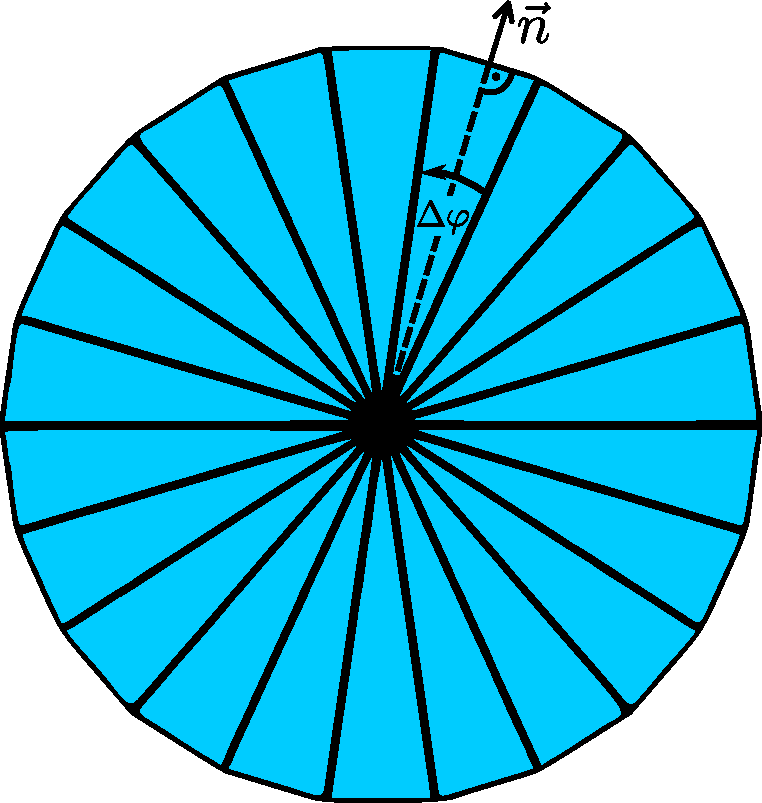
\includegraphics[height=4.5cm]{v1_zylinder1.pdf}
		\end{subfigure}
		\begin{subfigure}{0.49\textwidth}
			\centering
			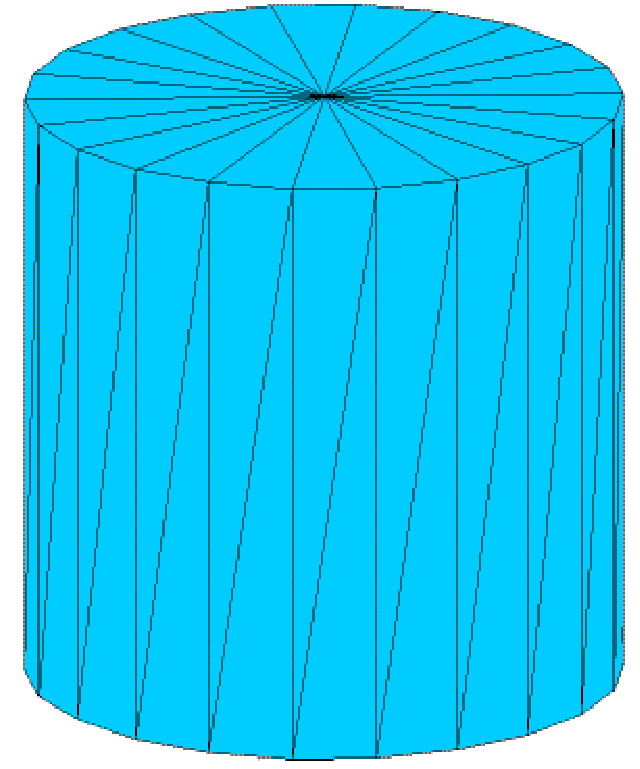
\includegraphics[height=4.5cm]{v1_zylinder2.pdf}
		\end{subfigure}
		\caption{Diskretisierung einer Kreiszylinderoberfläche. Dargestellt sind die Dreiecksgitter der Diskretisierung der Deckelfläche (links) und des diskretisierten Zylinders in Perspektivansicht (rechts).}\label{fig:zylGitter}
	\end{figure}



% --> Aufgabe
    \begin{framed}
	\noindent \textbf{7.} Überlegen Sie sich einen Pseudocode mit For-Schleifen, mit welchem Sie die Koordinaten aller Dreiecke der Oberflächendiskretisierung (siehe Abb.~\ref{fig:zylGitter}) bestimmen können. Die Anzahl der Dreiecke~$n_\text{D}$ soll dabei beliebig sein. Beachten Sie, dass zur Oberfläche Deck-, Mantel- und Bodenfläche gehören. Außerdem besitzen die Dreiecke auf der Mantelfläche \glqq unterschiedliche Orientierungen\grqq.\label{exer:pseudocodeCylinder}
\end{framed}

\emph{Fügen Sie hier Ihre Lösung ein}

% --> Aufgabe
    \begin{framed}
	\noindent \textbf{8.} In der Theorie wurde erwähnt, dass eine feinere Diskretisierung die Genauigkeit der Darstellung steigert\footnote{Es gibt jedoch Fälle, bei denen eine Verdichtung des Oberflächengitters nicht gegen die exakte Lösung konvergiert.}, aber dass auch der Rechenaufwand und der geforderte Speicher zunehmen.
        Berechnen Sie den Speicherplatz, der zur Speicherung des oben abgebildeten, diskretisierten Zylinders im STL-Format notwendig ist, als Funktion der Anzahl der Dreiecke $n_\mathrm{D}$ (Normalenvektoren müssen auch berücksichtigt werden). Beachten Sie hierbei lediglich die notwendige Anzahl der \lstinline{double}-Zahlen, wobei eine \lstinline{double}-Zahl \SI{8}{Byte} benötigt.\label{exer:requiredStorage}
\end{framed}

\emph{Fügen Sie hier Ihre Lösung ein}

% --> Aufgabe
    \begin{framed}
	\noindent \textbf{9.} Gegeben ist folgender Zusammenhang für die Fläche eines Deckflächendreieckes:
        \begin{align}
        A_\text{D} &= 2 \left[\frac12 a_\text{D} h_\text{D}\right] = 2 \left[ \frac12 \cdot r \cos\left(\frac{\Delta \varphi}{2}\right)\cdot r \sin\left(\frac{\Delta \varphi}{2}\right)  \right] = \frac12 r^2 \sin(\Delta\varphi)
        \end{align}
        Überlegen sie sich geometrisch, wie diese Formel zustande kommt und dokumentieren Sie die einzelnen Schritte. Leiten Sie anschließend eine Formel zur Berechnung des Volumens und der Fläche des gezeigten Zylinders in Abhängigkeit von der Anzahl der Deckflächendreiecke $n_\mathrm{D}$ her.\\
        Bestimmen Sie den relativen Oberflächenfehler $\Delta A$ bzw. Volumenfehler $\Delta V$ dieser Diskretisierung.
        Bei welchen Körpern wäre eine solche Oberflächendiskretisierung mit Dreiecken exakt?\label{exer:deltaAdeltaV}
\end{framed}

\emph{Fügen Sie hier Ihre Lösung ein}

% --> Aufgabe
    \begin{framed}
	\noindent \textbf{10.} Bei einigen Anwendungen ist es wichtig, dass die diskretisierte Fläche möglichst glatt bleibt. Ein
          wichtiges Beispiel hierbei ist die Streuung hochfrequenter elektromagnetischer Felder, wobei
          Kanten und Ecken das gestreute Feld verändern können. Angenommen bei der oberen
          Diskretisierung des Zylinders ist der Winkel zwischen den Normalenvektoren benachbarter Dreiecke der Deckflächen $\Delta \varphi \leq 5^{\circ}$ gefordert.
          Berechnen Sie die minimale Anzahl an Dreiecken zur Erfüllung dieser Forderung.\label{exer:smoothArea}
\end{framed}

\emph{Fügen Sie hier Ihre Lösung ein}



\section{Aufgaben während der Praktikumssitzung}
{\subsection{Differenzenverfahren}}

% --> Aufgabe
        \begin{framed}
	\noindent \textbf{1.} Implementieren Sie eine Methode
                    \begin{align}
                        \lstinline{[cc] = createCC(n, ord, bc)}\; \label{meth:createCC}
                    \end{align}     
                    welche die $\tilde{\textbf{C}}\textbf{C}$-Matrix mit der Stützstellenanzahl \lstinline{n}, der Ordnung des Differenzenverfahrens
                    \lstinline{ord}\\ (\lstinline{2} = zweite und \lstinline{4} = vierte Ordnung) und der für beide Ränder identischen Art der Randbedingung \lstinline{bc} (\lstinline{0=}fehlende, \lstinline{1=}elektrische und  \lstinline{2=}magnetische) erstellt.
                    Rückgabewert ist die $\tilde{\textbf{C}}\textbf{C}$-Matrix \lstinline{cc}. Nutzen Sie hierfür das vorgefertigte Template \lstinline{createCC.m}.\label{exer:createCC}
\end{framed}

\emph{Fügen Sie hier Ihre Lösung ein}

% --> Aufgabe
        \begin{framed}
	\noindent \textbf{2.} Ein einfacher Solver soll in
                    \begin{align}
                        \lstinline{[kx, modes] = solveCC(cc, dx)} \label{meth:solveCC}
                    \end{align}
                    implementiert werden, wobei die Schrittweite \lstinline{dx} als zusätzlicher Eingabeparameter übergeben wird.
                    \lstinline{kx} ist hier ein Vektor mit den geordneten Wellenzahlen, angefangen mit der kleinsten Wellenzahl. In gleicher
                    Reihenfolge sollen auch die Eigenvektoren in der Matrix \lstinline{modes} zurückgegeben werden.
                    Das Eigenwertproblem lässt sich durch die \matlab-Funktion \lstinline{eig} lösen, das Sortieren kann mit \lstinline{sort} erfolgen.\label{exer:solveCC}
\end{framed}

\emph{Fügen Sie hier Ihre Lösung ein}

% --> Aufgabe
        \begin{framed}
	\noindent \textbf{3.} Verwenden Sie die Routine \lstinline{createCC} mit \lstinline{n=6},~\lstinline{ord=2} und \lstinline{bc=0} und anschließend \lstinline{solveCC}.
                    Überprüfen Sie die Orthogonalität der Eigenvektoren. Wie viele Eigenmoden können bei dieser Parameterwahl bestimmt werden? Nutzen Sie hierfür die bereits gegebene Datei \lstinline{check_orth.m}.

                    {\textbf{Hinweis:}} Wenn Sie die Eigenvektoren geschickt miteinander multiplizieren, erhalten Sie eine Matrix, in der jeder Eintrag einem Produkt zweier Eigenvektoren entspricht. Diese sich ergebene Matrix lässt sich dann bequem mit dem Befehl \verb\imagesc\ (siehe Abschnitt~1.1.3) darstellen.\label{exer:check_orth}
\end{framed}

\emph{Fügen Sie hier Ihre Lösung ein}

% --> Aufgabe
        \begin{framed}
	\noindent \textbf{4.} Stellen Sie die zwei niedrigsten Moden in einem Skript \lstinline{plotModes} grafisch dar.
        Verwenden Sie \lstinline{n=100}, \lstinline{bc=1} und \lstinline{ord=4} sowie die Länge des eindimensionalen Gebietes L=\SI{5}{m}.\label{exer:plotModes}
\end{framed}

\emph{Fügen Sie hier Ihre Lösung ein}

% --> Aufgabe
        \begin{framed}
	\noindent \textbf{5.} Als nächstes sollen Sie das Konvergenzverhalten betrachten. Schreiben Sie ein Skript \lstinline{plotConv}, welches das Konvergenzverhalten in Abhängigkeit von der Stützstellenanzahl \lstinline{n}
                    Ihrer verschiedenen Implementierungen in zwei Grafiken dokumentiert:
                    \begin{enumerate}
                    \item Lineare Darstellung der Wellenzahl des Grundmodes über der Stützstellenanzahl $n$ im Fall elektrischer Randbedingungen, sowohl analytisch als auch zweite und vierte Ordnung.
                    \item Doppelt-logarithmische Darstellung des relativen Wellenzahlfehlers des Grundmodes  über die Gitterschrittweite bei elektrischen und fehlenden Randbedingungen für jeweils beide Ordnungen.
                    \end{enumerate}
                    Verwenden Sie die Grafiken um die Ordnung der verschiedenen Implementierungen graphisch zu bestimmen. Vergleichen Sie Ihr Ergebnis
mit Aufgabe~\ref{exer:failureTerm} aus der Vorbereitung.  Wie verändert sich das Konvergenzverhalten, wenn keine Randbedingungen implementiert sind?\label{exer:plotConv}
\end{framed}

\emph{Fügen Sie hier Ihre Lösung ein}



{\subsection{Dreidimensionale Darstellung}}

% --> Aufgabe
        \begin{framed}
	\noindent \textbf{6.} Schreiben Sie ein Skript \lstinline{plotCyl}, welches den Zylinder aus der Vorbereitung visualisiert.
Bauen Sie hierzu auf der \matlab-Funktion \lstinline{patch} auf. Verwenden Sie die Anzahl der Dreiecksflächen
                    in einer Deckelfläche \lstinline{nd=20}, den Radius \lstinline{r=1} und die Höhe \lstinline {h=1}.\label{exer:plotCyl}
\end{framed}

\emph{Fügen Sie hier Ihre Lösung ein}

% --> Aufgabe
        \begin{framed}
	\noindent \textbf{7.} Stellen Sie für einen Zylinder Ihrer Wahl den Oberflächenfehler $\Delta A$ sowie den Volumenfehler $\Delta V$ in Abhängigkeit von der Anzahl der Dreiecksflächen je Deckel $n_\text{D}$ (Vorbereitungsaufgabe \ref{exer:deltaAdeltaV}) in einem Skript
                    \lstinline{plotVisErr} doppelt-logarithmisch dar.   Mit welcher Ordnung konvergieren die Fehler?
                    Aus der Vorbereitung wissen Sie zusätzlich, wie der Speicherbedarf der
                    Darstellung skaliert.\\
                    Wie viele Dreiecke sind notwendig um einen Diskretisierungsfehler kleiner als $10^{-5}$ zu garantieren?\label{exer:plotVisErr}
\end{framed}

\emph{Fügen Sie hier Ihre Lösung ein}

% --> Aufgabe
      \begin{framed}
	\noindent \textbf{8.} Verwenden Sie die bereitgestellte Methode \lstinline{read_stl} um zwei der bereitgestellten Geometrien im STL-Format (vgl.~Abb.~1.4) einzulesen und dann erneut mit \lstinline{patch} darzustellen.
                Nennen Sie Ihr Skript \lstinline{plotStl}.\label{exer:plotStl}
\end{framed}

\emph{Fügen Sie hier Ihre Lösung ein}

%-------------------- Ende der Aufgaben --------------------

\section{Fazit}
\emph{Fügen Sie hier Ihre Lösung ein}

\end{document}
